\documentclass{ieeeaccess}
\usepackage{cite}
\usepackage{graphicx}
\usepackage{booktabs}
\usepackage{multirow}
\usepackage{url}

\begin{document}
\history{Supplementary material for review.}
\doi{}

\title{Supplementary Material: Detection and Tracking Diagnostics for Temporal Pixel Masking}
\author{Supplementary material for the submitted manuscript}
\maketitle

\section{Scope}

This supplement preserves object-detection diagnostics removed from the main manuscript and documents why tracking outputs are not reported as evidence. The experiments use one camera position and limited datasets, and they do not carry the primary conventional-OCR claim. Tracking was evaluated only with an in-project greedy associator after the official TrackEval path failed; those approximate scores are quarantined rather than compared as benchmark results.

\section{Real-Capture Object Detection and Tracking}
\label{sec:supp_real_detection}

To probe whether degradation extends beyond text, we ran an exploratory detection stress test within the same camera link. Content was displayed on the 240\,Hz screen, captured by the S600 at 1.5\,m / $0^{\circ}$, and processed by four detectors~\cite{b_yolo26,b_rtdetr2024,b_fasterrcnn2015,b_retinanet2017}. Mean average precision (mAP), mAP at 0.50 intersection over union (mAP50), and average recall (AR) are reported descriptively. The protected condition uses the $n=4$ mask+noise profile without overlays or inversion. The \texttt{real\_clean} reference is an unprotected nominal 31.25-ms capture. The \texttt{real\_short} image is the maximum-grayscale-contrast frame from a three-frame protected burst at the nominal 3.91-ms setting; this rule was implemented before detector inference but was not preregistered. The \texttt{real\_video} image is the mean of 150 protected frames acquired nominally at 60\,fps. Protection, exposure, resolution, and frame reduction are therefore confounded in cross-condition comparisons.

\begin{table}[!t]
\caption{Real-Capture COCO Detection Diagnostics (150 Images; Nominal UVC Control Labels). Conditions Differ in Protection, Exposure, Resolution, and Frame Reduction and Do Not Estimate a Protection Effect.}
\label{tab:supp_real_coco}
\centering
\footnotesize
\begin{tabular}{llccc}
\toprule
Detector & Condition & mAP & mAP50 & AR \\
\midrule
\multirow{3}{*}{YOLO26x}
 & real\_clean & 28.6\% & 43.9\% & 31.0\% \\
 & real\_short & 1.3\% & 2.4\% & 1.4\% \\
 & real\_video & 3.5\% & 5.3\% & 3.6\% \\
\midrule
\multirow{3}{*}{RT-DETR-x}
 & real\_clean & 30.1\% & 50.2\% & 34.8\% \\
 & real\_short & 3.5\% & 5.8\% & 4.1\% \\
 & real\_video & 4.6\% & 7.3\% & 5.5\% \\
\midrule
\multirow{3}{*}{Faster R-CNN}
 & real\_clean & 21.3\% & 39.2\% & 28.7\% \\
 & real\_short & 0.8\% & 1.6\% & 0.9\% \\
 & real\_video & 1.5\% & 3.0\% & 1.8\% \\
\midrule
\multirow{3}{*}{RetinaNet}
 & real\_clean & 22.6\% & 39.4\% & 27.0\% \\
 & real\_short & 0.9\% & 1.8\% & 1.0\% \\
 & real\_video & 1.9\% & 3.1\% & 2.0\% \\
\bottomrule
\end{tabular}
\end{table}

Across the four detectors, mAP50 is 39.2--50.2\% for \texttt{real\_clean}, 1.6--5.8\% for \texttt{real\_short}, and 3.0--7.3\% for \texttt{real\_video} (Fig.~\ref{fig:supp_real_det_drop}). These are exposure-confounded descriptive diagnostics, not protection effects. A separate 450-frame MOT17-09-FRCNN still-display collection was processed with a greedy ByteTrack-inspired associator. Because it was neither continuous synchronized video nor evaluated through official ByteTrack/TrackEval, its HOTA/IDF1-like outputs are not reported.

\begin{figure}[!t]
\centering
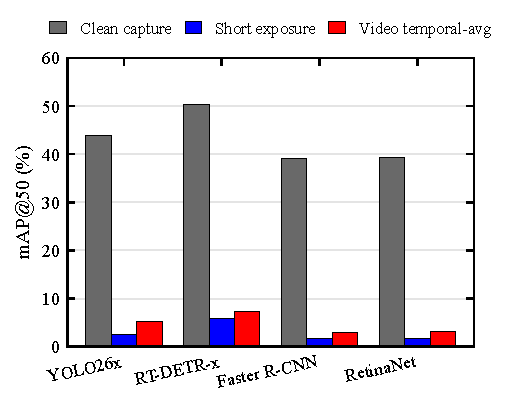
\includegraphics[width=\columnwidth]{figures/real_detection_drop.pdf}
\caption{Descriptive mAP50 across three exposure-confounded real-capture conditions. Differences cannot be attributed to protection alone.}
\label{fig:supp_real_det_drop}
\end{figure}

\section{Software Detection and Tracking Simulation}
\label{sec:supp_sim_detection}

Supplementary simulations were run on 8 Common Objects in Context (COCO) val2017 images~\cite{b_coco2014} with YOLO26x~\cite{b_yolo26}, RT-DETR-x~\cite{b_rtdetr2024}, Faster R-CNN~\cite{b_fasterrcnn2015}, and RetinaNet~\cite{b_retinanet2017}. Table~\ref{tab:supp_coco_sim} is an implementation diagnostic, not a dataset-level estimate. A separate multiple-object-tracking MOT17~\cite{b_mot16} simulation used an in-project greedy association fallback after TrackEval failed. Its approximate tracking outputs are omitted because they are not equivalent to official ByteTrack/TrackEval results.

\begin{table}[!t]
\caption{COCO val2017 Simulated Detection Pipeline Diagnostics (4 Detectors, 8 Images; Not a Dataset-Level Performance Estimate)}
\label{tab:supp_coco_sim}
\centering
\footnotesize
\setlength{\tabcolsep}{5.8pt}
\begin{tabular}{llccc}
\toprule
Detector & Condition & mAP & mAP50 & AR \\
\midrule
\multirow{3}{*}{YOLO26x}
 & clean & 48.1\% & 58.3\% & 51.0\% \\
 & single subframe & 0.0\% & 0.0\% & 0.0\% \\
 & temporal avg. & 14.3\% & 18.3\% & 14.3\% \\
\midrule
\multirow{3}{*}{RT-DETR-x}
 & clean & 47.1\% & 58.7\% & 53.4\% \\
 & single subframe & 5.2\% & 6.0\% & 5.2\% \\
 & temporal avg. & 16.8\% & 23.7\% & 17.9\% \\
\midrule
\multirow{3}{*}{Faster R-CNN}
 & clean & 38.2\% & 52.7\% & 43.6\% \\
 & single subframe & 3.0\% & 4.4\% & 3.0\% \\
 & temporal avg. & 11.1\% & 16.5\% & 11.1\% \\
\midrule
\multirow{3}{*}{RetinaNet}
 & clean & 33.2\% & 47.1\% & 35.3\% \\
 & single subframe & 3.3\% & 4.2\% & 3.3\% \\
 & temporal avg. & 9.6\% & 13.2\% & 9.6\% \\
\bottomrule
\end{tabular}
\end{table}

On these 8~images, single-subframe mAP50 across four detectors is 0--6.0\%. This sample is sufficient only to check pipeline behavior, not to estimate COCO performance. Differences among detectors may reflect architecture, thresholds, proposal density, or implementation details; the experiment does not isolate those factors.

\bibliographystyle{IEEEtran}
\bibliography{refs}
\EOD

\end{document}
